\chapter{Getting Started}
\addtocontents{toc}{\protect\setcounter{tocdepth}{2}}
\hypersetup{bookmarksdepth=5}

\section{Keyboard}
\label{cha:getting-started}
\index{Keyboard}

Now that everything is connected, it's time to get familiar with the MEGA65 keyboard.

You may notice that the keyboard is a little different to the keyboards used on computers today. While most keys will be in familiar positions, there are some specialised keys, and some with special graphic symbols marked on the front.

The graphic symbols are typable in some display modes, similar to letters, numbers, and punctuation. The complete set of characters is known as the {\em PETSCII character set}.\index{PETSCII}

\subsection{Special Keys}

\subsubsection{RETURN}
\index{Keyboard!RETURN}
Pressing \specialkey{RETURN} enters the information you have typed into the MEGA65's memory. The computer will either act on a command, store some information, or display an error message if you made a mistake.

\subsubsection{SHIFT}
\index{Keyboard!Shift Keys}
The two \specialkey{SHIFT} keys are located on the left and the right. They work very much like the Shift key on a regular keyboard. They also perform some special functions as well.

In upper case mode, holding down \specialkey{SHIFT} and pressing any key with two graphic symbols on the front produces the right-hand symbol on that key. For example, \specialkey{SHIFT} and \megakey{J} prints the \graphicsymbol{J} character.

In lower case mode, pressing \specialkey{SHIFT} and a letter key prints the upper case letter on that key.

To type the Greek letter $\pi$ (pi), hold \specialkey{SHIFT} and press \megakeywhite{$\uparrow$}.

Holding \specialkey{SHIFT} down and pressing a Function key accesses the function shown on the front of that key. For example: \specialkey{SHIFT} and \megakey{F1} activates \megakey{F2}.


\subsubsection{SHIFT LOCK}
\index{Keyboard!SHIFT LOCK}
In addition to \specialkey{SHIFT} is \specialkey{SHIFT\\LOCK}. Press this key to lock down the Shift function. Now any key you press while \specialkey{SHIFT\\LOCK} is illuminated prints the character to the screen as if you were holding down \specialkey{SHIFT}. This includes special graphic characters.

\subsubsection{CTRL}
\index{Keyboard!CTRL}
\specialkey{CTRL} is the Control key. Holding down \specialkey{CTRL} and pressing another key allows you to perform Control functions. For example, holding down \specialkey{CTRL} and one of the number keys (from \megakey{1} to \megakey{8}) allows you to change text colours. The colour that is printed at the top row on the front of the number key will be used. Holding down \specialkey{CTRL} and pressing \megakey{9} or \megakey{0} switches reverse-text mode on and off.

There are some examples of this on page \pageref{sec:screen-editor}, and all of the Control functions are listed on page \pageref{appendix:controlcodes}.

If a program is being {\bf LIST}ed to the screen, holding down \specialkey{CTRL} slows down the display of each line. You can read more about the {\bf LIST} command on page \pageref{BASIC 65 Commands!LIST}.\index{BASIC 65 Commands!LIST}

Holding \specialkey{CTRL} and pressing \megakey{*} enters the Matrix Mode Debugger (refer to the {\bf MEGA65 Book} for more details).

\subsubsection{RUN STOP}
\index{Keyboard!RUN STOP}
Normally, pressing \specialkey{RUN\\STOP} stops the execution of a program. Holding \specialkey{SHIFT} while pressing \specialkey{RUN\\STOP} {\bf RUN}s the first program from disk.\index{BASIC 65 Commands!RUN}

Some programs override the \specialkey{RUN\\STOP} key and cannot be stopped in this way.

You can boot your MEGA65 into the {\bf Machine Code Monitor}\index{Machine Code Monitor} by holding down \specialkey{RUN\\STOP} and pressing reset on the left-hand side of the computer.

\subsubsection{RESTORE}
\index{Keyboard!RESTORE}
The computer screen can be restored to a clean state without clearing the memory by holding down \specialkey{RUN\\STOP} and pressing \widekey{RESTORE}. This combination also resets operating system vectors and re-initialises the screen editor, which makes it a handy combination if the computer has become a little confused.

Some programs override the \specialkey{RUN\\STOP} + \widekey{RESTORE} key combination and cannot be reset in this way.

You can also enter the {\bf Freezer} by pressing and holding \widekey{RESTORE} for one second, then releasing the key. You can
read more about the Freezer on page \pageref{sec:freezer}.\index{Freezer menu}

\subsubsection{THE CURSOR KEYS}
\index{Keyboard!Cursor Keys}
\nopagebreak
At the bottom right-hand side of the keyboard are the cursor keys. These four directional keys allow you move the cursor to any position for on-screen editing.

The cursor moves in the direction indicated on the keys: \megakey{$\leftarrow$} \megakey{$\uparrow$} \megakey{$\rightarrow$} \megakey{$\downarrow$}.

You don't have to keep pressing a cursor key over and over. If you need to move the cursor a long way, you can keep the key pressed down. When you are finished, simply release the key.

\subsubsection{ARROW KEYS}
\index{Keyboard!Arrow Keys}
These keys are different to the cursor keys! They are \megakeywhite{$\leftarrow$} (next to \megakey{1}), and \megakeywhite{$\uparrow$} (next to \widekey{RESTORE}).
Both arrow keys are used in various BASIC functions and escape sequences.

For example, \megakeywhite{$\leftarrow$} can be used as a shortcut for {\bf SAVE},\index{BASIC 65 Commands!SAVE} and \megakeywhite{$\uparrow$} is used to raise a number to a power (which is the same as multiplying a number by itself a specified number of times).

You can read more about the available escape sequences on page \pageref{escape-sequences}.

These two PETSCII specific keys will always be shown in MEGA65 literature with a white background.

It is also possible to move the cursor up by using \specialkey{SHIFT} and \megakey{$\downarrow$}, and left by using \specialkey{SHIFT} and \megakey{$\rightarrow$}. This owes to the MEGA65's Commodore 64 heritage, which only had two cursor keys.

\subsubsection{INSerT/DELete}
\index{Keyboard!INST DEL}
The \specialkey{INST\\DEL} key, the rightmost key of the top row, is the INSERT / DELETE key. When you press \specialkey{INST\\DEL}, the character to the left is deleted, and all characters to the right are shifted one position to the left.

To insert a character, hold \specialkey{SHIFT} and press \specialkey{INST\\DEL}. All the characters to the right of the cursor are shifted to the right. This allows you to type a letter, number or any other character at the newly inserted space.


\subsubsection{CLeaR/HOME}
\index{Keyboard!CLR HOME}
The \specialkey{CLR\\HOME} is the CLEAR / HOME key. Pressing \specialkey{CLR\\HOME} places the cursor at the top left-most position of the screen.

Holding down \specialkey{SHIFT} and pressing \specialkey{CLR\\HOME} clears the entire screen {\it and} places the cursor at the top left-most position of the screen.

If you press \specialkey{CLR\\HOME} accidentally, you can return the cursor to its prior position by pressing \specialkey{ESC} then \specialkey{CLR\\HOME}.

\subsubsection{MEGA KEY}
\index{Keyboard!MEGA Key}
\megasymbolkey or the MEGA key provides a number of different functions and can be used to launch special utilities.

Holding \specialkey{SHIFT} and pressing \megasymbolkey switches between lower and uppercase character modes.

Holding \megasymbolkey and pressing any key with two graphic symbols on the front prints the left-most graphic symbol to the screen. For example,
\megasymbolkey and \megakey{D} prints the \graphicsymbol{d} symbol.

Holding \megasymbolkey and pressing a number key switches to a secondary colour, i.e., the colour that is printed at the bottom row on the front of the number key.

Holding \megasymbolkey and pressing \specialkey{TAB} enters the Matrix Mode Debugger (refer to the {\bf MEGA65 Book} for more details).

Switching on the MEGA65 or pressing the reset button on the left-hand side while holding down \megasymbolkey switches the MEGA65 into GO64 mode.\index{Commodore 64!GO64 mode}

\subsubsection{NO SCROLL}
\index{Keyboard!NO SCROLL}
If a program is being {\bf LIST}ed to the screen, pressing \specialkey{NO\\SCROLL} pauses the screen output. Press any key to un-pause.

This feature is not available in GO64 mode.\index{Commodore 64!GO64 mode}

\subsubsection{FUNCTION KEYS}
\index{Keyboard!Function Keys}
There are seven Function keys available for use by software applications. \megakey{F1} \megakey{F3} \megakey{F5} \megakey{F7} \megakey{F9} \megakey{F11} and \megakey{F13} can be used to perform special functions.

Hold \specialkey{SHIFT} to access \megakey{F2} through to \megakey{F14} as shown on the front of each Function key.
\index{Keyboard!Shift Keys}
Only Function keys \megakey{F1} to \megakey{F8} are available in GO64 mode.\index{Commodore 64!GO64 mode}

\subsubsection{HELP}
\index{Keyboard!HELP}
\specialkey{HELP} can be used by software, and also acts as \megakey{F15}.

\subsubsection{ALT}
\index{Keyboard!ALT}
Holding \specialkey{ALT} down while pressing other keys can be used by software to perform specific functions. This feature is not available in GO64 mode.\index{Commodore 64!GO64 mode}

Holding \specialkey{ALT} down while switching the MEGA65 on activates the Utility Menu.\index{Utility menu} You can format an SD card, or enter the MEGA65 Configuration Utility\index{Configuration!Utility} to select the default video mode and change other settings, or test your keyboard.

\subsubsection{CAPS LOCK}
\index{Keyboard!CAPS LOCK}
\specialkey{CAPS\\LOCK} works similarly to \specialkey{SHIFT\\LOCK} in C65 and MEGA65-modes, but only modifies the letter keys.

When the MEGA65 is set to run at a reduced processor speed, such as in GO64 mode,\index{Commodore 64!GO64 mode} you can hold down \specialkey{CAPS\\LOCK} to run the processor at full speed temporarily. This is useful in GO64 mode for things such as
speeding up loading from the internal disk drive or SD card, or to greatly speed up the de-packing process after a program is run. MEGA65 mode runs at maximum speed by default.

\addtocontents{toc}{\protect\setcounter{tocdepth}{5}}


\section{The Screen Editor}
\label{sec:screen-editor}

When you switch on your MEGA65 or reset it, the following screen will appear:\footnote{This assumes you have disabled the Intro Disk menu. If the Intro Disk menu is running, press ``/'' (forward slash) to exit to this screen.}

\begin{center}
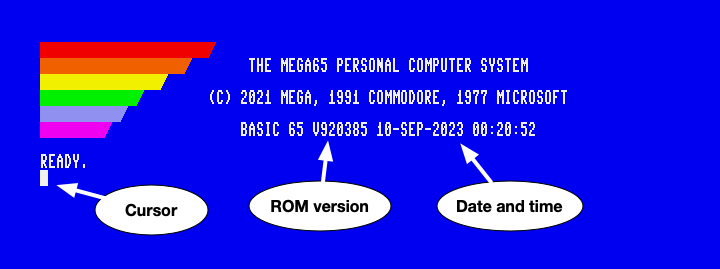
\includegraphics[width=0.9\linewidth]{images/introduction-screen/layout.png}
\end{center}

The colour bars in the top left-hand side of the screen can be used as a guide to help calibrate the colours of your display. The screen also displays the name of the system, the copyright notice, and the ROM version. The displayed date and time are taken from the internal RTC (Real-Time Clock) at the time the computer was powered on. You can set the date and time in the Configuration Utility.

Finally, you will see the \screentext{READY} prompt and the flashing cursor.

You can begin typing keys on the keyboard and the characters will be printed at the cursor position. The cursor itself will advance after each key press.

You can also produce reverse text or colour bars by holding down \specialkey{CTRL} and pressing \megakey{9}, or \megakey{R}. This enters reverse text mode. When this is enabled, you can press and hold the \megakey{Space} bar. While doing so, a white bar will be drawn across the screen.
\index{Keyboard!CTRL}
You can change the current colour by holding \specialkey{CTRL} down and pressing a number key (from \megakey{1}
to \megakey{8}). For example, if you press and hold \specialkey{CTRL} down and press \megakey{1}, the colour will
change to black. Now, when you hold down the \megakey{Space} bar, a black bar will be drawn. If you continue to
change the colour and press the \megakey{Space} bar, you will get an effect similar to the following image:

\begin{center}
\includegraphics[width=0.7\linewidth]{images/introduction-screen/colour-bars.png}
\end{center}

You can disable reverse text mode by holding \specialkey{CTRL} and pressing \megakey{0}.

A further eight colours can be selected by holding down \megasymbolkey and pressing a key from \megakey{1} to \megakey{8}.\index{Keyboard!MEGA Key}

The colour that is printed at the bottom row on the front of the number key will be used. For example, if you held
\megasymbolkey down while pressing \megakey{4}, dark grey will be used. For access to an additional 16 colours of the alternate/rainbow palette, refer to the \specialkey{CTRL} + \megakey{A} shortcut described on page \pageref{appendix:controlcodes}.

\underline{NOTE}:
\begin{itemize}
  \item {\bf Quote Mode}: If you were to press \megakey{"} to open a string, and then try to change
colours, reverse text, move the cursor keys, or use the \specialkey{CLR\\HOME} key, instead
of these actions instantly occurring, funny PETSCII\index{PETSCII} symbols will appear instead. This is
due to a BASIC facility called {\it quote mode},
which allows you to encode such actions into a string so that they can be executed at a later
time (for example, via a {\bf PRINT} statement within your programs). To end {\it quote mode}, simply
type another \megakey{"} to mark the end of your string.
  \item {\bf Insert Mode}: A similar facility is called
{\it insert mode}, where for the number of times you press \specialkey{SHIFT} + \specialkey{INST\\DEL}
to insert a few spaces, the same number of keypresses that follow it will abide by the same
principles of {\it quote mode}.
  \item You can forcefully exit either of these modes by pressing \specialkey{ESC}, \megakey{O}.
\end{itemize}

\needspace{4cm}
You can create fun pictures just by using these colours and letters. Here's an example of what a 4th year student drew:

\begin{center}
\includegraphics[width=0.7\linewidth]{images/caleb-PETSCII-TNT-final}
\end{center}

What will you draw?

\needspace{2cm}
\textbf{Functions}

Functions using \specialkey{CTRL} are called \textbf{Control Codes}.
Functions using \megasymbolkey are called \textbf{Mega Codes}. There are also functions that are called by using \specialkey{SHIFT}, which are called \textbf{Shifted Codes}.

Lastly, \specialkey{ESC} enables the use of \textbf{Escape Sequences}.

You can read about all of these functions in detail on page \pageref{appendix:controlcodes}.

\needspace{2cm}
\textbf{ESC Sequences}

\index{Keyboard!Escape Sequences}
Escape sequences are performed a little differently than a Control function or a Shift function. Instead of holding the modifier key down, an Escape sequence is performed by pressing \specialkey{ESC} and releasing it, followed by pressing the desired key.

For example: to switch between 80 column mode and 40 column mode, press and release \specialkey{ESC}, then press \megakey{X}.

There are more text modes available. You can create flashing text by holding \specialkey{CTRL} down and pressing \megakey{O}. Any characters you type in will flash. Turn flash mode off by pressing \specialkey{ESC}, then \megakey{O}.


\section{Editor Functionality}

The MEGA65 screen editor\index{Screen editor} supports several ways to quickly move the cursor around the screen to help you to be more productive.

For example, press \specialkey{CLR\\HOME} to go to the home position on the screen. Hold \specialkey{CTRL} down and press \megakey{W} several times. This is the \textbf{Word Advance function}, which jumps your cursor to the next word, or printable character.

You can set custom tab positions on the screen for your convenience. Press \specialkey{CLR\\HOME} and then \megakey{$\rightarrow$} to move the cursor to the fourth column. Hold down \specialkey{CTRL} and press \megakey{X} to set a tab. Move another 16 positions to the right, and press \specialkey{CTRL} and \megakey{X} again to set a second tab.

Press \specialkey{CLR\\HOME} to go back to the home position. Hold \specialkey{CTRL} down and press \megakey{I}. This is the \textbf{Forward Tab function}. Your cursor will tab to the fourth position. Press \specialkey{CTRL} and \megakey{I} again. Your cursor will move to position 8. By default, every 8th position is already set as a tabbed position. So the 4th and 20th positions have been added to the existing tab positions. You can continue to press \specialkey{CTRL} and \megakey{I} to advance to the 16th and 20th positions.

\subsection{Creating a Window}
\index{Keyboard!Escape Sequences}
\index{Windows!Escape sequences}

You can set a window on the MEGA65 working screen. Move your cursor to the beginning of the "BASIC 65" text. Press \specialkey{ESC}, then press \megakey{T}. Move the cursor 10 lines down and 15 to the right.

Press \specialkey{ESC}, then \megakey{B}. Anything you type will be contained within this window.

For example, if you were to type \screentext{LIST} to list out a program, the listing will be confined to the window region you have specified:

\begin{center}
\includegraphics[width=0.7\linewidth]{images/set-window.png}
\end{center}

To escape from the window back to the full screen, press \specialkey{CLR\\HOME} twice.

\subsection{Additional ASCII characters}

You may have noticed a few ASCII characters on the MEGA65 keyboard that aren't traditionally a part of the PETSCII character set\index{PETSCII}. To use these characters:

\begin{itemize}
  \item Type either \screentext{FONT A} or \screentext{FONT B}.
  \item Press \megasymbolkey + \specialkey{SHIFT} to switch to lowercase.
\end{itemize}

You will now be able to type those additional ASCII characters by holding \megasymbolkey and pressing the key.

\begin{center}
  \begin{tabular}{|l|c|l|}
  \hline
  \textbf{Name} & \textbf{Symbol} & \textbf{Key} \\
  \hline
  Backtick & \texttt{\`} & \megasymbolkey + \megakeywhite{$\leftarrow$} \\
  \hline
  Tilde & \texttt{\~} & \megasymbolkey + \megakey{,} (comma) \\
  \hline
  Vertical bar & \texttt{|} & \megasymbolkey + \megakey{.} (period) \\
  \hline
  Backslash & \texttt{\textbackslash} & \megasymbolkey + \megakey{/} \\
  \hline
  Left curly bracket & \texttt{\{} & \megasymbolkey + \megakey{:} \\
  \hline
  Right curly bracket & \texttt{\}} & \megasymbolkey + \megakey{;} \\
  \hline
  Underscore & \texttt{\_} & \megasymbolkey + \megakey{=} \\
  \hline
  \end{tabular}
\end{center}

The alternate fonts replace characters from the original PETSCII character set with these symbols. To revert back to the PETSCII character set, type \screentext{FONT C}.

\subsection{Uppercase and lowercase}

\megasymbolkey + \specialkey{SHIFT} switches between uppercase and lowercase text for the entire display. This works even during program execution, so you can adjust it if a program is in the wrong mode.


\section{The Freezer Menu}
\label{sec:freezer}
\index{Freezer menu}
\nopagebreak
The MEGA65 spends most of its time behaving as a Commodore 65 computer would, either running a program or awaiting instructions in the BASIC environment. Your MEGA65 has additional features that were not part of the original C65 design. You can access many of these features from the Freezer menu.

To open the Freezer menu, hold the \widekey{RESTORE} key for one second, then release it. The MEGA65 will pause whatever it is doing, flicker the border colour, then open the Freezer menu. Whatever program was running remains in memory and can be resumed by pressing the \megakey{F3} key. You can also abandon the running program and reset the MEGA65 by pressing \megakey{F5}.

\begin{center}
  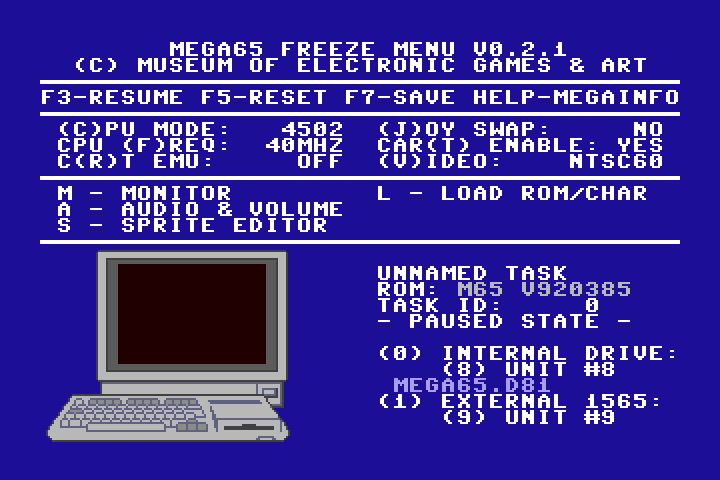
\includegraphics[width=0.7\linewidth]{images/freezer.png}
\end{center}

One feature to remember when playing games is the ``(J)OY SWAP.'' This causes the two joystick ports to trade numbers. If you have a joystick in port 2 and you start a game that expects a joystick in port 1, instead of disconnecting and reconnecting the joystick, open the Freezer menu, press \megakey{J} to swap the port numbers, then resume your game.

This is called the ``Freezer'' menu because the state of the MEGA65 remains frozen while using it. The Freezer menu can store multiple freeze states, and you can switch between them. To save the current state, navigate to an unused {\it freeze slot} using the cursor-right key, then press \megakey{F7}. When the border stops blinking, the state is saved. To restore a state, navigate to the freeze slot, then press \megakey{F3} to resume operation.

The Freezer menu has several built-in options and features. For more information about the MEGA65 Information Utility (``MEGAINFO''), see ``Determining the Versions of Things'' on page \pageref{sec:versions}. For more information about mounting disks and disk images, see chapter \vref{cha:using-disks}.


\section{Running Commodore 64 Software}

The MEGA65 is capable of running Commodore 64 software. There are two ways to do this: the built-in GO64 mode, and the {\it C64 for MEGA65} FPGA core.

\subsection{GO64 Mode}
\index{Commodore 64!GO64 mode}

The original Commodore 65 was designed to be capable of running some Commodore 64 software. The MEGA65 supports this feature, known as ``GO64 mode.''

\underline{NOTE}: Due to how Commodore designed this feature, not all C64 software is compatible with this mode. Unlike the similar feature of the Commodore 128, the Commodore 65 uses a different CPU, and minor differences are known to cause compatibility issues with some software titles.

There are three ways to switch the MEGA65 into GO64 mode:

\begin{itemize}
    \item Switch off the computer, hold the \megasymbolkey and switch it back on.
    \item From the MEGA65 \screentext{READY} prompt, enter this command: \screentext{GO64} Enter \screentext{YES} when prompted.\index{BASIC 65 Commands!GO64}
    \item Switch off the computer, connect a Commodore 64 cartridge to the expansion port, then switch the computer on.
\end{itemize}

\begin{center}
  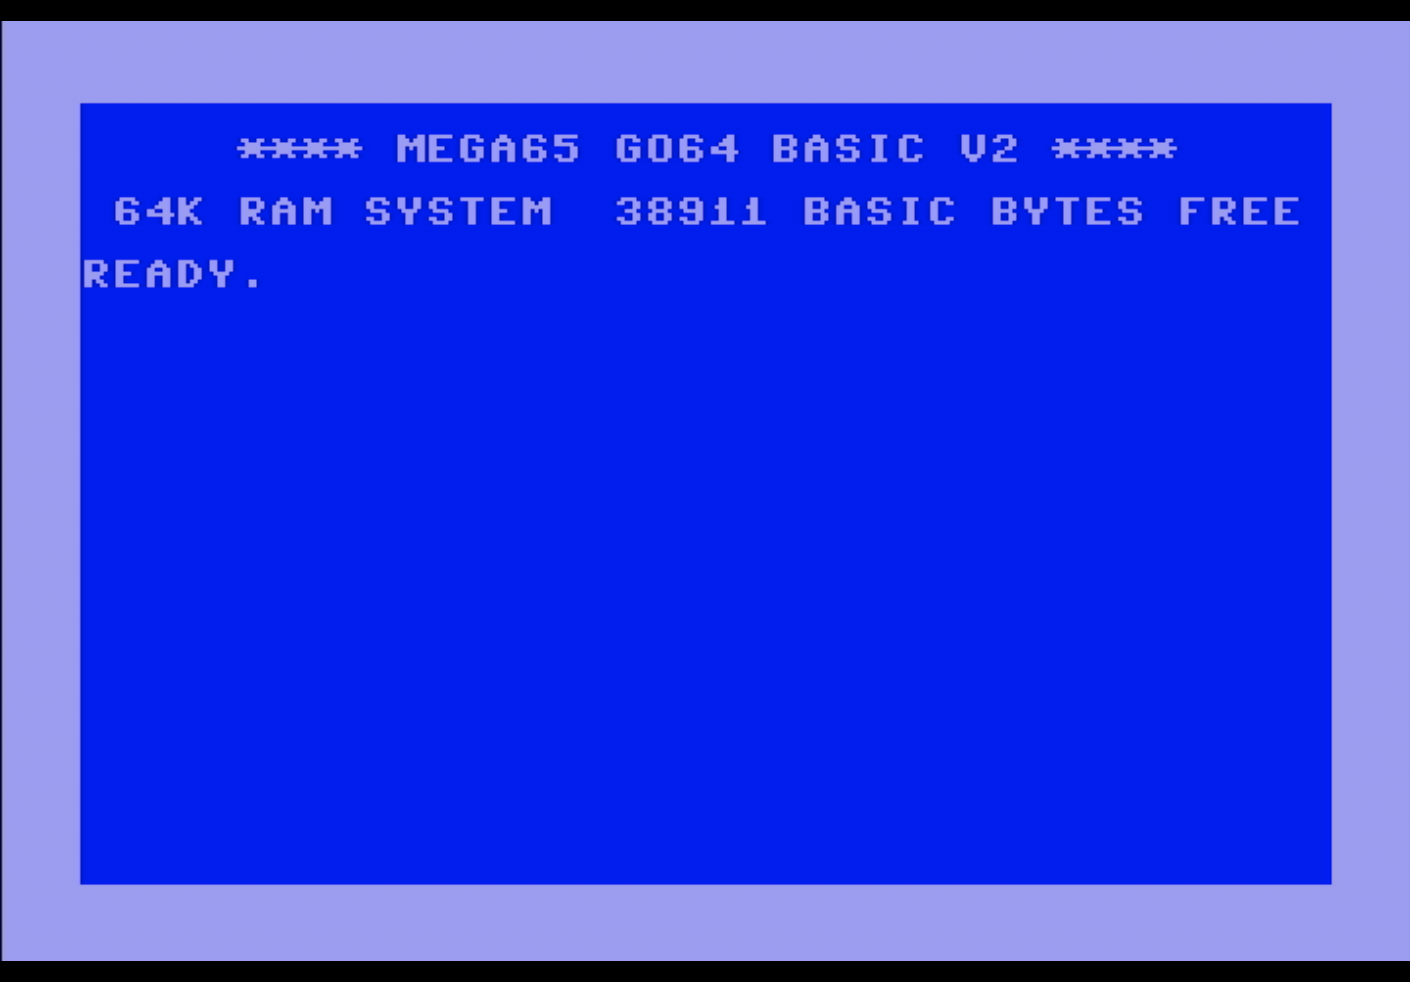
\includegraphics[width=0.7\linewidth]{images/go64.png}
\end{center}

GO64 mode is actually just a temporary re-configuration of the MEGA65. All of the MEGA65's features are still present, including the Freezer menu for mounting D81 disk images.

Much Commodore 64 software can be found on the Internet in the form of D64 disk images. The MEGA65 only supports D81 disk images via the SD card and Freezer menu. You can use a peripheral such as the SD2IEC\index{SD2IEC device} with the MEGA65's IEC port to use D64 disk images. Be sure to obtain an SD2IEC with an independent power supply, and not one that depends on a Commodore 64 tape connector.\footnote{For more information on SD2IEC devices, see: \url{https://www.c64-wiki.com/wiki/SD2IEC}}

\subsection{The ``C64 for MEGA65'' FPGA Core}
\index{Core!C64 core}\index{Commodore 64!Core}

The {\it C64 for MEGA65} FPGA core by MJoergen and sy2002 re-creates the original Commodore 64 computer on MEGA65 hardware with a high degree of accuracy. It does so by completely replacing the MEGA65 core with one that implements the Commodore 64 chipset, including its CPU. MEGA65 features such as the Freezer menu are not available when running the C64 core. Instead, the core provides its own menu for mounting D64 disk images and other features. Press the \specialkey{HELP} key with the core running to access this menu.

% TODO: When the cartridge-to-core configuration feature is complete:
% With the C64 core installed, you can configure the MEGA65 boot process to use the core when a Commodore 64 cartridge is connected, instead of using the less-compatible GO64 mode. ...
% (Refer to chapter \vref{cha:cores})

For information about installing FPGA cores, see chapter \vref{cha:cores}. To download the {\it C64 for MEGA65} core and read important installation instructions, see: \url{https://github.com/MJoergen/C64MEGA65}
